%%%%% USEFUL MACROS
%
% PROBABILITY
% Expectation:  \E
% Probability:  \Pr
% Variance:     \Var
% KL Div:       \Div{}{}        % looks like D( - || - )
%
% LINEAR ALGEBRA
% Matrix (bf):  \mat{}
% Vector (bf):  \vec{}
%
% ANALYSIS
% Abs:          \abs{}
% Norm:         \norm{}
% Inner prod:   \ip{}
% Argmin:       \argmin{}
% Argmax:       \argmax{}
% Varepsilon:   \eps
%
% COMMON SETS
% Reals:        \bbR
% Rationals:    \bbQ
% Naturals:     \bbN
% Complex Num:  \bbC
% Integers:     \bbZ
% Finite field: \bbF

% Contributors: Vincent Liu, Yadin Rozov, Laura Tinsi
Unsupervised learning begins with the assumption that given a dataset
$\mathcal{X}$, there exists an underlying structure. Our learning task
is to discover this structure given a relatively small amount of data.
One of the most intuitive concepts of a structure is a
cluster---groups of points that behave similarly to each other, but
quite differently to points in other clusters

To warm up, we can ask a few questions:
\begin{itemize}
\item \emph{What is clustering?} Given input
  data, a clustering algorithm partitions the data into multiple
  `meaningful' groups. 
\item \emph{Why do we need it?} If we can cluster similar points
  together, we can approximate large/infinite/continuous set of
  objects with a finite set of representatives.
\item \emph{What are its applications?} Briefly, applications include
  vector quantization, codebook learning, dictionary learning. It is
  also used in computer vision to map from pixel space to HOG
  (histogram of oriented gradient) space to give rise to new
  features.
\item \emph{How do we cluster?} There are three main types of
    clustering methods. The first that we study is \textit{centroid}
    based clustering, such as Lloyd's Algorithm, where we try to
    identify central vectors that represent each cluster. Another 
    type is \textit{density} based clustering, such as DBSCAN
    where clusters are identified as areas where data points are
    densely located. The last is \textit{proximity} based, such as
    spectral clustering, where we first construct a graph with our
    dataset and estimate a partition.
\end{itemize}
In short, clustering aims to find a meaningful way to group
datapoints, which is especially important in exploratory data
analysis, helping us understand and summarize input data.


\section{Metric space preliminaries}
\begin{definition}[Metric space]
Let $\mathcal{X}$ be a space and $\rho: \mathcal{X} \times \mathcal{X}
\to \mathbb{R}$ a function. A \emph{metric space} is a pair
$(\mathcal{X},\rho)$ such that $\rho$ satisfies the following:
\begin{itemize}
\item non-negativity (reflexivity): $\forall x,y \in \mathcal{X},
  \rho(x,y) \ge 0$ with equality iff $x=y$ 
\item symmetry: $\forall x,y \in \mathcal{X}, \rho(x,y) = \rho(y,x)$ 
\item triangle inequality: $\forall x,y,z \in \mathcal{X}, \rho(x,y)
  \le \rho(x,z) + \rho(z,y)$. 
\end{itemize}
We call $\rho$ a \emph{metric} or a \emph{distance function}.

\end{definition}

We should be cautious about symmetry: there are instances where
the distances are not necessarily symmetric. For example, if we are
clustering facility locations, since there are one-way roads,
distances between facilities need not be symmetric.

Given a metric space $\mathcal{X}$, we can define the distance between
a point and a subset $T$ of $\mathcal{X}$: 
\begin{definition}
For a set $T \subset \mathcal{X}$, we define: 
\[\rho(s,T) := \inf_{t\in T} \rho(s,t)\]
\end{definition}

\begin{example} Let $\mathcal{X} = \mathbb{R}^d$. Here are a few
familiar metrics on $\mathcal{X}$:
\begin{itemize}
\item $\ell_2$ distance on $\mathbb{R}^d$: $\forall x,y$,
\[\ell_2(x,y) = \rho(x,y) = \sqrt{\sum_{i=1}^d (x_i - y_i)^2}\] 
\item $\ell_1$  distance on $\mathbb{R}^d$: $\forall x,y$, 
\[\ell_1(x,y) = \rho(x,y) = \sum_{i=1}^d |x_i - y_i|\]
\item $\ell_\infty$ distance on $\mathbb{R}^d$: 
\[\ell_{\infty} = \max_i |x_i - y_i|\]
\end{itemize}
\end{example}

\begin{example}[Geodesics] In a nonlinear space (i.e. a manifold),
the distance between two points is defined as the shortest path
between those two points. If the manifold may be embedded into a
Euclidean space, note that the shortest path on the manifold may
not leave the manifold. We also called this path the shortest 
geodesic.
\end{example}
\begin{figure}
    \centering
    \captionsetup{width=0.8\textwidth}
    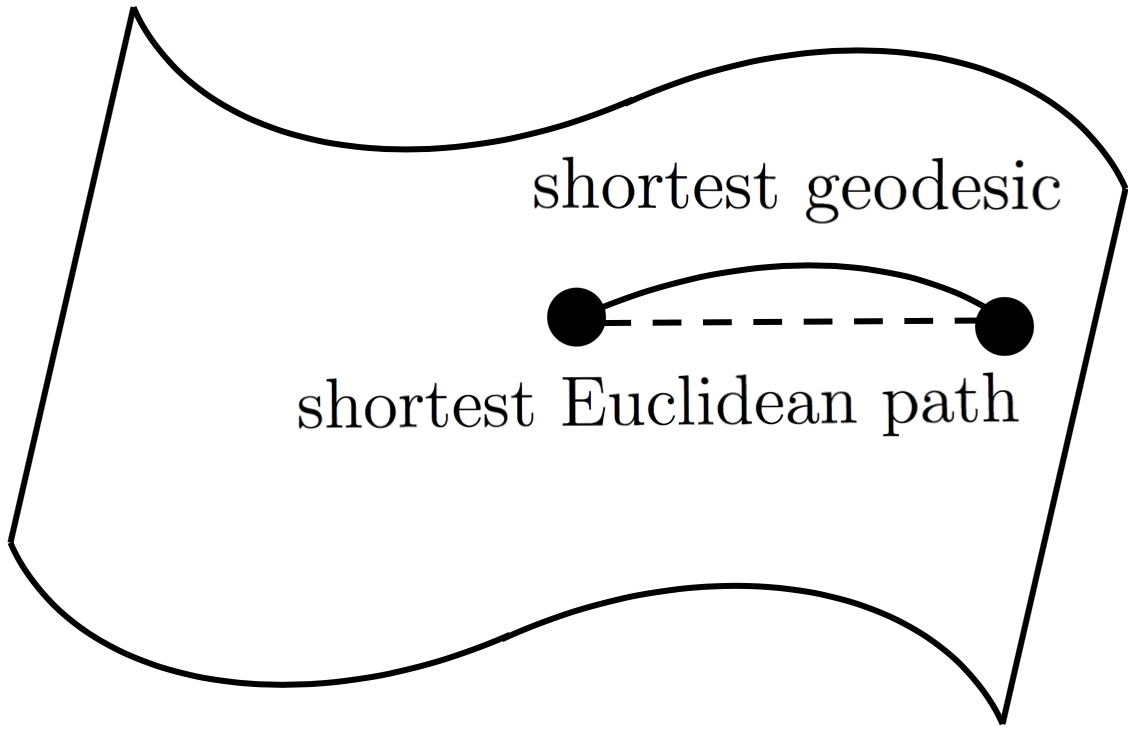
\includegraphics[scale=0.3]{chapter_1/files/geodesic.jpg}
    \caption{A manifold $\mathcal{M}$ embedded in some Euclidean
    space $\mathbb{R}^n$ may have a shortest geodesic that is
    not the same as the shortest Euclidean path.}
    \label{fig:geodesic}
\end{figure}
\begin{example}[Graph metric] The shortest path on graphs (for 
example a social network graph) forms a valid distance function. The
distance is just the smallest number of edges between two vertices, 
and defined as $\infty$ for vertices that cannot reach each other.
\end{example}
\begin{remark}
A metric space isn't always a Euclidean space. So, we cannot always
perform Euclidean operations (i.e. taking the mean) in an arbitrary
metric space.
\end{remark}

A metric gives a space a notion of distance or similarity. A natural
concept of a \emph{covering} helps us give a space a notion of size.

\begin{definition}[Cover]
Let $S \subset \mathcal{X}$, $\epsilon \geq 0$. A set $T \subset
\mathcal{X}$ is an $\epsilon$-cover of $S$ if:  $\forall s \in S$,
$\exists t \in T$ s.t. $\rho(s,t) \le \epsilon$.
\end{definition}

In other words, $T$ $\epsilon$-covers $S$ if $\sup_{s\in S} 
\rho(s,T)\leq \epsilon$.

\begin{exercise}
(i) Is $S$ a cover of $S$? (ii) Given the vertices of a $d$-dimensional
cube $\{-1,1\}^d$ the $\ell_\infty$ distance. What is a good 1-cover?
$\frac{1}{2}$-cover? $\frac{9}{10}$-cover?
\end{exercise}

\begin{enumerate}[(i)]
	\item $S$ is a $\epsilon$-cover of $S$ for all $\epsilon \geq 0$,
	as for every element $x_i \in S$, $\rho(x_i, x_i) = 0 \leq 
	\epsilon$.
	
	\item It is clear that a good 1-cover for $S = \{-1, 1\}^d$ with 
	$\rho = \ell_\infty$ would be the set $\{\vec{0}\}$. However, for 
	an $\epsilon$-cover with $\epsilon < 1$, the smallest cover is of 
	size $2^d$. The proof is as follows:
	
	\begin{proof}
		Let $T'$ be an $\epsilon$-cover of $S$ that contains less than
		$2^d$ elements. Then, $\exists\ x, x' \in S, t \in T$ such that 
		both $\rho(x, t) < \epsilon$ and $\rho(x', t) < \epsilon$. We 
		know that the distance between any two vertices of the unit 
		hypercube is equal to 2. However, when we apply the triangle
		inequality:
		\begin{align*}
			\rho(x, x') & = 2\\
			\rho(x, t) + \rho(x', t) & \geq \rho(x, x')\\
			& \geq 2
		\end{align*}
		Which implies that either $\rho(x, t) \geq 1$ or $\rho(x', t) 
		\geq 1$, contradicting our earlier claim that both $\rho(x, t) 
		< \epsilon$ and $\rho(x', t) < epsilon$. Thus, the smallest
		possible $\epsilon$-cover of $S$ for $\epsilon < 1$ is of size
		$2^d$.
	\end{proof}
\end{enumerate}

\begin{exercise}
	Let $D=[0,1]^d$ with the Euclidean metric and let $N_\epsilon(d)$ be the smallest number of
	points required to form an $\epsilon$-cover of $D$. What is the asymptotic behavior of $N_\epsilon(d)$ in the variable $d$? 
	Hint: consider filling $D$ with d-dimensional balls.
\end{exercise}
